\documentclass[a4paper]{article}
\usepackage[spanish]{babel}
\usepackage[utf8]{inputenc}
\usepackage{charter}   % tipografia
\usepackage{graphicx}
%\usepackage{makeidx}
\usepackage{paralist} %itemize inline

\usepackage{color} % para snipets de codigo coloreados
\usepackage{fancybox}  % para el sbox de los snipets de codigo

\definecolor{litegrey}{gray}{0.94}

% \newenvironment{sidebar}{%
% 	\begin{Sbox}\begin{minipage}{.85\textwidth}}%
% 	{\end{minipage}\end{Sbox}%
% 		\begin{center}\setlength{\fboxsep}{6pt}%
% 		\shadowbox{\TheSbox}\end{center}}
% \newenvironment{warning}{%
% 	\begin{Sbox}\begin{minipage}{.85\textwidth}\sffamily\lite\small\RaggedRight}%
% 	{\end{minipage}\end{Sbox}%
% 		\begin{center}\setlength{\fboxsep}{6pt}%
% 		\colorbox{litegrey}{\TheSbox}\end{center}}

\newenvironment{codesnippet}{%
	\begin{Sbox}\begin{minipage}{\textwidth}\sffamily\small}%
	{\end{minipage}\end{Sbox}%
		\begin{center}%
		\vspace{-0.4cm}\colorbox{litegrey}{\TheSbox}\end{center}\vspace{0.3cm}}




\usepackage{fancyhdr}

\pagestyle{fancy}

\renewcommand{\sectionmark}[1]{\markright{\thesection\ - #1}}

\fancyhf{}

\fancyhead[LO]{Sección \rightmark} % \thesection\ 
\fancyfoot[LO]{\small{Leandro Raffo, Maximiliano Fernández Wortman, Uriel Rozenberg.}}
\fancyfoot[RO]{\thepage}

\renewcommand{\headrulewidth}{0.5pt}
\renewcommand{\footrulewidth}{0.5pt}
\setlength{\hoffset}{-0.8in}
\setlength{\textwidth}{16cm}
%\setlength{\hoffset}{-1.1cm}
%\setlength{\textwidth}{16cm}
\setlength{\headsep}{0.5cm}
\setlength{\textheight}{25cm}
\setlength{\voffset}{-0.7in}
\setlength{\headwidth}{\textwidth}
\setlength{\headheight}{13.1pt}

\renewcommand{\baselinestretch}{1.1}  % line spacing




% \setcounter{secnumdepth}{2}

\usepackage{caratula}


\begin{document}


\thispagestyle{empty}
\materia{Organización del Computador II}
\submateria{Segundo Cuatrimestre de 2015}
\titulo{Trabajo Práctico II}
\subtitulo{Programacion SIMD}
\integrante{Leandro Raffo}{}{}
\integrante{Maximiliano Fernández Wortman}{}{}
\integrante{Uriel Rozenberg}{}{}

%Pagina de titulo e indice
%\thispagestyle{empty}

\maketitle 

\tableofcontents

\newpage

\section{Introduccion}
En este trabajo práctico realizamos la implementación de dos filtros de imagenes, con tal de ver que tan eficiente puede llegar a ser (o no) SIMD, los filtros son la diferencia de imagenes y el blur gaussiano, los cuales fueron implementados en lenguaje C (gcc y clang) y assembly, haciendo uso de instrucciones vectoriales. Luego comparamos la performance de estas implementaciones sobre diferentes imagenes y usando herramientas probabilísticas y estadísticas.

\section{Implementacion}

\subsection{Diferencia}
\noindent Descripcíon de un ciclo de la iteración del filtro diferencia.\\
Primermo pedimos memoria para declarar las máscaras que vamos a usar y armamos el stackframe (omitido)
\begin{codesnippet}
\begin{verbatim}
section .rodata
mask_5 DB 2,2,2,2,6,6,6,6,10,10,10,10,14,14,14,14
trans_2 DB 0,0,0,255,0,0,0,255,0,0,0,255,0,0,0,255
\end{verbatim}
\end{codesnippet}

\noindent Luego de armar el stackframe tenemos
\begin{codesnippet}
\begin{verbatim}
mov r12, rdx
mov eax, r8d
mov ecx, ecx
mul rcx
xor r15, r15
\end{verbatim}
\end{codesnippet}
r12 apunta a la matriz resultado, ecx tiene la cantidad de filas, y la parte baja de rax tiene la cantidad de columnas. Al hacer mul rcx se tiene filas*columnas en rdx:rax, como las operaciones son de 32 bits tenemos la multiplicación en rax, que es lo que vamos a usar, junto a r15 para iterar. Ahora entramos al ciclo.

\begin{codesnippet}
\begin{verbatim}
.ciclo:
    cmp r15, rax
    JE .fin
\end{verbatim}
\end{codesnippet}

\noindent Comparamos si r15 es igual a rax en tal caso ya hicimos la diferencia sobre todos los pixeles y termina el ciclo. El ciclo sigue con

\begin{codesnippet}
\begin{verbatim}
    movdqu xmm3 , [RDI +  r15*4]   
    movdqu xmm15, [RSI +  r15*4]
    movdqu xmm14, xmm15     
    pminub xmm15, xmm3        
    pmaxub xmm3 , xmm14        
    psubb  xmm3 , xmm15             
    movdqu xmm4, xmm3 
    movdqu xmm5, xmm3       
\end{verbatim}
\end{codesnippet}

\noindent Movemos a xmm$3$ los primeros $4$ pixeles de la primera matriz y a xmm$15$ los primeros $4$ de la segunda matriz a comparar, estos ocupan respectivamente $16$ bytes en memoria (brga por $4$). Después Guardamos en xmm$14$ el valor de xmm$15$ y hacemos un pminub entre xmm$15$ y xmm$3$ lo cual deja en xmm$15$ el mínimo byte a byte. Lo mismo para xmm$3$ pero con pmaxub es decir este tiene el máximo byte a byte. Hacemos esto porque queremos calcular el valor absoluto de la forma $|x-y|$ = $\max(x,y) - \min(x,y)$. Concluimos esta idea haciendo psubb entre xmm$3$ que tenia el máximo y xmm$15$ que tenia el mínimo y finalmente guardamos el resultado en xmm$4,5$ para operar en la siguiente parte.

\begin{codesnippet}
\begin{verbatim}
    pslldq xmm4, 1                  
    pslldq xmm5, 2               
    movdqu xmm6, xmm5             
    pmaxub xmm6, xmm4             
    pmaxub xmm6, xmm3              
    pshufb xmm6, [mask_5] 
    paddsb xmm6, [trans_2]
    movdqu [r12 +  r15*4], xmm6
    add  r15d, 4
    jmp .ciclo
\end{verbatim}
\end{codesnippet}
\noindent Ahora shifteamos con packed shift xmm$4,5$ uno y dos bytes respectivamente de forma de poder tomar el máximo de entre r g b en paralelo, es decir $4$ pixels a la vez. Por ejemplo, el primer byte de xmm$4$ tiene al byte de r, y el de xmm$6$ tiene al byte de g, de forma que al hacer pmaxub entre  xmm$6$ y xmm$4$ nos deja en el primer byte de xmm$6$ (y cada 3 bytes) max(r$_n$,g$_n$) donde $n = \{1,2,3,4 \}$ indican los pixeles que levantamos. Los demas bytes de este registro no nos interesan. Repetimos esto entre xmm$6$ y xmm$3$, pasa de vuelta lo mismo pero ahora tenemos en el primer byte de xmm$6$ (y cada $3$ bytes) max(r$_n$,g$_n$,b$_n$) con $n = \{1,2,3,4 \}$. Ahora tenemos que mover este máximo a las 3 coordenadas r, g y b, hacemos esto mediante la mascara mask$_5$ y mediante trans$_2$ sumamos con saturación con tal de dejar en alpha el valor $255$. Copiamos los 16 bytes correspondientes (con el offset adecuado) en la matriz destino, sumamos $4$ a r$15$d y saltamos para, si es necesario, volver a hacer el ciclo completo.

\subsection{Blur gaussiano}

\noindent En el blur gaussiano calculamos 4 pixeles por iteración, pero para legibilidad solo vamos a escribir lo que le pasa a uno solo, se repite el código y se apunta a memoria correctamente. 

\begin{codesnippet}
\begin{verbatim}
movdqu xmm0,[r12]  
movdqu xmm1, xmm0
punpckhbw xmm0, xmm7 
punpcklbw xmm1, xmm7  
movdqu xmm2, xmm0
movdqu xmm3, xmm1
punpckhwd xmm0, xmm7  	
punpcklwd xmm2, xmm7   
punpckhwd xmm1, xmm7  
punpcklwd xmm3, xmm7  
\end{verbatim}
\end{codesnippet}

\noindent Primero levantamos $16$ bytes de memoria, equivalente a $4$ pixeles en xmm$0$ y lo copiamos en xmm$1$ ya que vamos a desempaquetar los datos. Llamamos a punpcklbw/hbw junto a un xmm$7$ que estaba en $0$, tenemos entonces que xmm$0$ tiene los primeros $2$ pixeles ($8$ bytes) extendidos a cada uno a un word. Lo mismo para xmm$1$. Luego repetimos el proceso desempaquetando a un double word, ya que queremos operar con floats y este es su tamaño. 

\begin{codesnippet}
\begin{verbatim}
cvtdq2ps xmm0,xmm0
\end{verbatim}
\end{codesnippet}

\noindent Convertimos a float 




\section{Resultados}

\subsection{Diferencia}

Para analizar las implementaciones de C y assembly, corrimos  cada implementación de diferencia sobre una imagen de $2308$x$2308$ con un tamaño de $16$mb, las implementaciones de C se compilaron con gcc y clang usando los flags de optimización -O0, -O1, -O2 y -O3
\begin{figure}
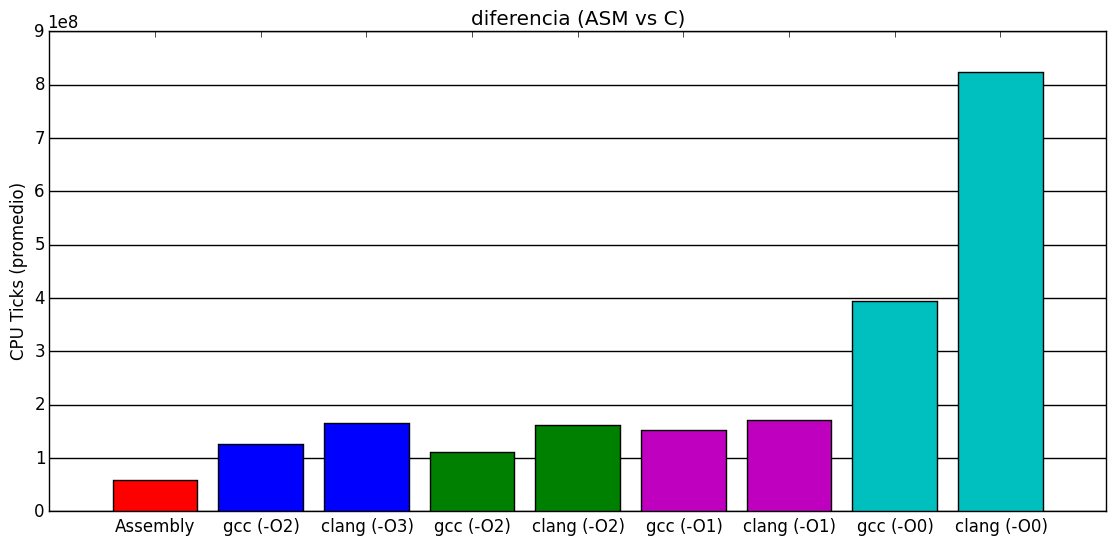
\includegraphics[scale=0.52]{diferenciaCvsASM_Intel_E8440.png}
\caption{Promedio sobre una imagen de $2308$x$2308$}
\end{figure}



\subsection{Blur}

\section{Conclusión}

\end{document}